%% ===========================================================================
%% GENERATED FILE — template: arxiv-custom
%%
%% Rewritten by `make set-template PAPER=<doc> TEMPLATE=<name>`. Hand edits are
%% detected (the pristine hash is recorded in .template.yml) and the switch will
%% refuse rather than discard them — but they still belong in the template
%% source, tools/templates/arxiv-custom/main.tex.
%%
%% Your writing is NOT here. It lives in:
%%   metadata.tex   title, authors, affiliations, keywords
%%   abstract.tex   the abstract
%%   text.tex       every section
%%   acronyms.tex   acronym definitions
%%
%% arxiv-custom.sty is OURS: tools/templates/arxiv-custom/arxiv-custom.sty is the
%% editable source, copied here by `make sync-bib`. Change the source, never the
%% copy. See tools/templates/arxiv-custom/README.md for how it differs from
%% upstream, and ../../AGENTS.md for the generated-file contract.
%% ===========================================================================
\documentclass{article}

%% Our patched arxiv style. Loads geometry and fancyhdr itself — do not
%% re-import either of them below.
\usepackage{arxiv-custom}

\usepackage[T1]{fontenc}
\usepackage[utf8]{inputenc}
\usepackage{microtype}
\usepackage{amsmath}
\usepackage{amsfonts}
\usepackage{amssymb}
\usepackage{nicefrac}
\usepackage{graphicx}
\usepackage[table]{xcolor}
\usepackage{booktabs}
\usepackage{enumitem}
\usepackage{url}

\graphicspath{{figures/}{./}}

%% Citations: natbib in every template, so \citep and \citet work identically
%% whichever template the document uses and text.tex stays portable.
\usepackage{natbib}

%% Document metadata — title, authors, keywords.
%%
%% THIS FILE IS YOURS. It is deliberately template-agnostic: `make set-template`
%% rewrites main.tex but never touches this file, so switching between IEEE and
%% arXiv formats keeps your title and author list.
%%
%% Each template composes these macros into its own author block, because
%% \IEEEauthorblockN and authblk have nothing in common. Adding an author means
%% uncommenting the macros below AND adding one line to main.tex — see
%% tools/templates/README.md, "Author blocks".

\newcommand{\PaperTitle}{An Example Paper for the Paper Template}

%% Running head. Keep it short — it has to fit across the page.
\newcommand{\PaperShortTitle}{Paper Template}

%% Comma-separated. Used for \IEEEkeywords and arxiv.sty's \keywords.
\newcommand{\PaperKeywords}{reproducibility, research infrastructure, LaTeX}

%% PDF subject line — arXiv categories work well here, e.g. cs.LG, cs.AI.
\newcommand{\PaperSubject}{cs.DL}

%% Flat author list for the PDF metadata.
\newcommand{\PaperAuthorList}{Author Name}

%% --- Authors ----------------------------------------------------------------
\newcommand{\AuthorOneName}{Author Name}
\newcommand{\AuthorOneAffil}{Institution}
\newcommand{\AuthorOneEmail}{author@example.org}
\newcommand{\AuthorOneOrcid}{https://orcid.org/0000-0000-0000-0000}

% \newcommand{\AuthorTwoName}{Second Author}
% \newcommand{\AuthorTwoAffil}{Institution}
% \newcommand{\AuthorTwoEmail}{second@example.org}
% \newcommand{\AuthorTwoOrcid}{https://orcid.org/0000-0000-0000-0000}

% \newcommand{\AuthorThreeName}{Third Author}
% \newcommand{\AuthorThreeAffil}{Institution}
% \newcommand{\AuthorThreeEmail}{third@example.org}
% \newcommand{\AuthorThreeOrcid}{https://orcid.org/0000-0000-0000-0000}

\usepackage{researchcommon}

%% Acronyms — load order is load-bearing, all before hyperref.
\usepackage[acronym,nopostdot,nonumberlist]{glossaries-extra}
\makenoidxglossaries
\RestoreAcronyms
\setacronymstyle{long-short}
% Acronym definitions for this document.
%
% Define acronyms HERE, never inline in the body. In prose use \gls{key} /
% \glspl{key} mid-sentence and \Gls{key} / \Glspl{key} at sentence start.
% In section titles wrap them: \texorpdfstring{\gls{key}}{SHORT}.
%
% Do NOT glossarify proper names (DINOv2, PyTorch, ...) or affiliations.

\newacronym{rl}{RL}{reinforcement learning}
\newacronym{mfec}{MFEC}{Model-Free Episodic Control}
\newacronym{nec}{NEC}{Neural Episodic Control}
\newacronym{vit}{ViT}{Vision Transformer}


\usepackage[hidelinks]{hyperref}
%% `doi` loads hyperref itself, with no options — it must come AFTER our
%% optioned \usepackage[hidelinks]{hyperref} or LaTeX raises an option clash.
\usepackage{doi}
\usepackage{cleveref}

\renewcommand{\headeright}{Preprint}
\renewcommand{\undertitle}{Preprint}
\renewcommand{\shorttitle}{\PaperShortTitle}

\hypersetup{
  pdftitle={\PaperTitle},
  pdfauthor={\PaperAuthorList},
  pdfsubject={\PaperSubject},
  pdfkeywords={\PaperKeywords},
}

\title{\PaperTitle}
\date{}   % remove to print today's date under the author block

%% Author block: authblk with ORCID icons, multi-affiliation variant. To add an
%% author, uncomment their macros in metadata.tex and repeat the \author[1]{...}
%% line; \affil[n] numbers the affiliations.
\usepackage{authblk}
\renewcommand\Authfont{\bfseries}
\setlength{\affilsep}{0.5em}
\newbox{\orcid}\sbox{\orcid}{
\includegraphics[scale=0.06]{orcid.pdf}}

\author[1]{%
  \href{\AuthorOneOrcid}{\usebox{\orcid}~\AuthorOneName\thanks{\texttt{\AuthorOneEmail}}}%
}
\affil[1]{\AuthorOneAffil}

\begin{document}

\maketitle

\begin{abstract}
  %% The abstract, prose only — no \begin{abstract}, the template supplies that.
%% THIS FILE IS YOURS: `make set-template` never touches it.

This is the worked example shipped with the paper template. It exists to prove
that one command fetches experiment results from the tracker, regenerates every
figure and table from them, and compiles this document---so that a number in a
paper always has a traceable path back to the runs that produced it. Replace
this paper with your own; the wiring is the point.

\end{abstract}

\keywords{\PaperKeywords}

%% The body of the paper — every section lives here.
%%
%% THIS FILE IS YOURS. `make set-template` rewrites main.tex but never touches
%% this file, so the same prose compiles under every template. Two rules keep
%% that true (see tools/templates/README.md):
%%
%%   * cite with \citep / \citet — every template loads natbib
%%   * anything you \begin{} must come from researchcommon.sty, not from one
%%     template's preamble

\section{Introduction}
\label{sec:introduction}

Experiment code and the paper written about it normally live in separate
repositories, and the numbers travel between them by hand. They then go stale
silently: nothing connects the figure in the PDF to the runs it summarizes, and
a table copied out of a notebook keeps its authority long after the sweep that
produced it was rerun. This repository closes that gap without merging the two
codebases: the paper fetches its numbers from the experiment tracker, records
which runs it fetched, and fails to build when the two disagree.

\begin{contributions}
\item A committed, human-readable cache of experiment-tracker results, with
  the exact run identifiers behind it pinned in a lockfile, so a paper's
  numbers are reproducible without access to the tracker.
  \label{c:cache}
\item Figures and tables generated from that cache with recorded provenance,
  which makes staleness a build failure rather than a reading error.
  \label{c:provenance}
\item A document directory that compiles standalone---on Overleaf, and as a
  flattened submission bundle---and whose prose survives a change of venue
  template.
  \label{c:portable}
\end{contributions}

\section{Method}
\label{sec:method}

% NOTE: `% NOTE:` comments are author instructions for prose that is planned but
% not yet written. Agents must treat the nearest NOTE as the specification for
% what belongs there, and must never delete or rewrite one. See ../../AGENTS.md.

% NOTE: describe the actual method here. This placeholder section exists only so
% the example compiles to a plausible short paper.

The synthetic study behind \cref{fig:learning_curve} stands in for a real
experiment. Deep reinforcement learning from pixels \citep{mnih2015human} is
sample-inefficient, which motivated episodic control methods
\citep{blundell2016modelfree,pritzel2017neural}. \citet{oquab2024dinov2} showed
that self-supervised features transfer broadly; replacing an episodic
controller's state encoder with such features is the kind of question this
repository layout is built to support.

\begin{figure}[!t]
  \centering
  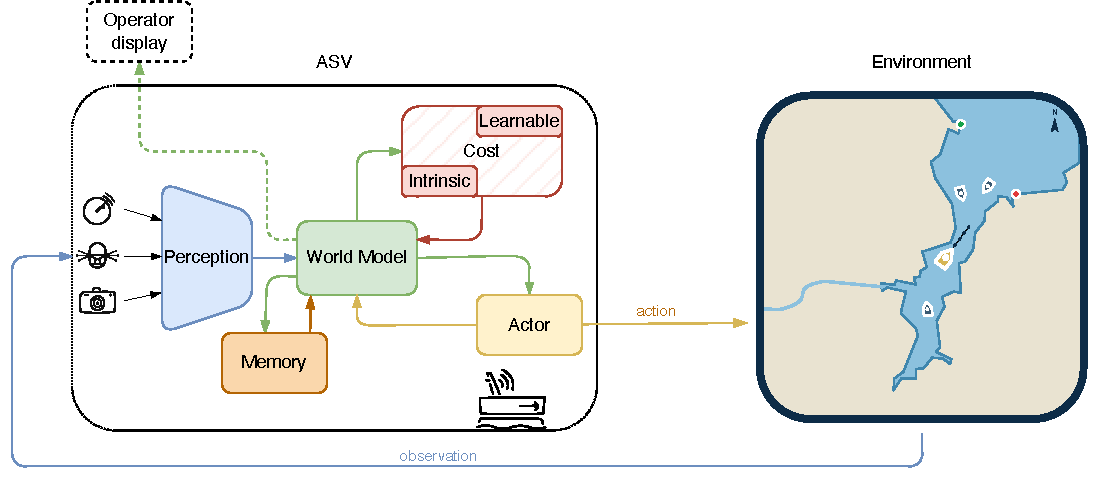
\includegraphics[width=\linewidth]{architecture.pdf}
  \caption{Example schematic: a world-model control loop. The source is
    \texttt{figures/architecture.drawio}; regenerate the export with
  \texttt{make drawio}.}
  \label{fig:architecture}
\end{figure}

Hand-authored diagrams live beside the data-figure configs, as
\texttt{.drawio} sources. \Cref{fig:architecture} is one: it is drawn by hand,
not fetched from the tracker, and its PDF is a generated export.

\section{Results}
\label{sec:results}

Neither \cref{fig:learning_curve} nor \cref{tab:final_scores} is drawn or typed
by hand. Both are rendered from \texttt{data/learning\_curves.csv} and
\texttt{data/final\_scores.csv}, which \texttt{make fetch} writes from the runs
pinned in \texttt{data/wandb.lock.yml}. Each output records the content hash of
the file it read, so changing the data without rebuilding fails
\texttt{make check-generated} instead of quietly shipping a stale result.

\begin{figure}[!t]
  \centering
  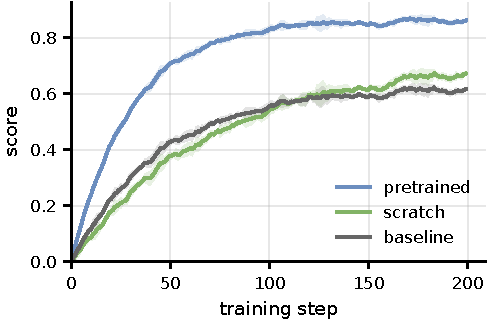
\includegraphics[width=\linewidth]{learning_curve.pdf}
  \caption{Learning curves for the synthetic example study: mean over five
    seeds, shaded band is one standard deviation. Regenerate with
  \texttt{make plots}.}
  \label{fig:learning_curve}
\end{figure}

\begin{table}[!t]
  \centering
  \caption{Final score after training, mean over five seeds. The tabular is
  generated; the caption, label and float placement are not.}
  \label{tab:final_scores}
  %% GENERATED FILE — do not edit.
%%
%% Written from tables/final_scores.yml
%% out of the committed W&B cache. Rebuild with: make tables
%%
%% Editing this file by hand puts the paper's numbers out of step with the
%% runs behind them, and `make check-generated` will not catch it — it checks
%% the inputs, not the output. Change the config instead.
%%
%% This is a bare tabular: wrap it in \begin{table} with your caption and
%% label in text.tex.

\begin{tabular}{lrrr}
\toprule
Method & Score & SD & Seeds \\
\midrule
pretrained & 0.86 & 0.01 & 5 \\
scratch & 0.67 & 0.01 & 5 \\
baseline & 0.62 & 0.01 & 5 \\
\bottomrule
\end{tabular}

\end{table}

\begin{figure}[!t]
  \centering
  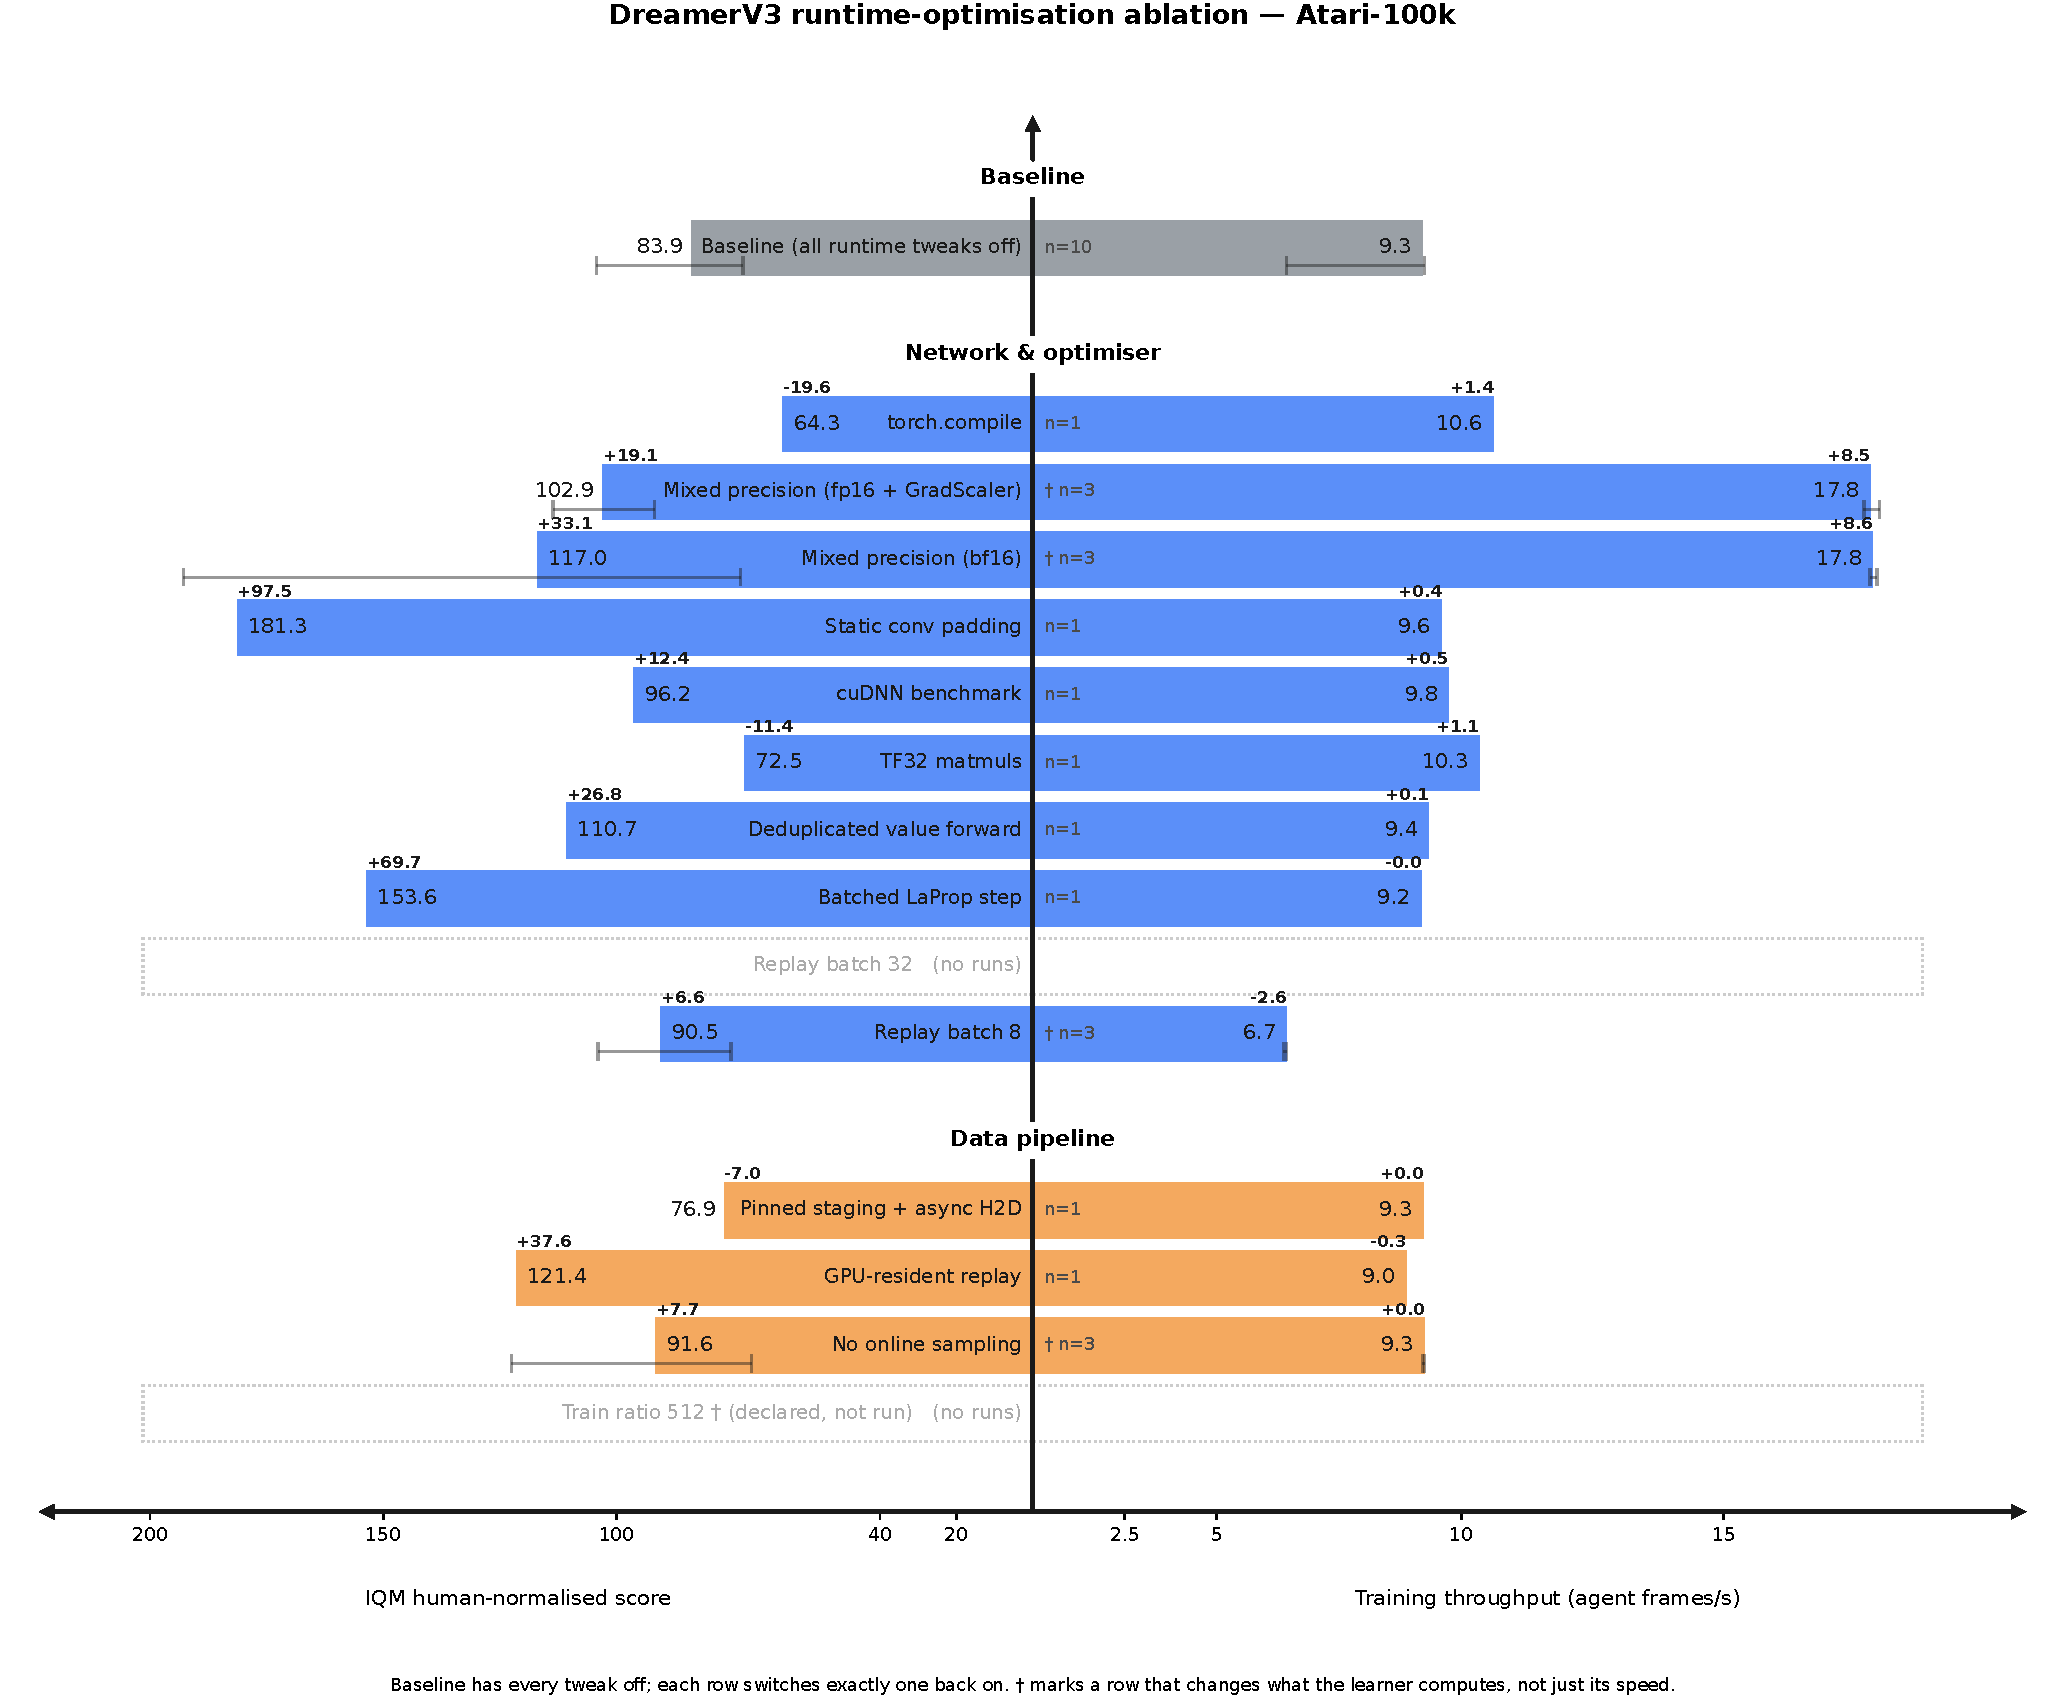
\includegraphics[width=\linewidth]{dreamer_optimisations_ablation.pdf}
  \caption{DreamerV3 runtime-optimisation ablation on Atari-100k. Rendered from
    \texttt{data/figures/dreamer\_optimisations\_ablation.csv}, pinned to the
  runs in \texttt{data/wandb.lock.yml}. Regenerate with \texttt{make plots}.}
  \label{fig:dreamer_optimisations_ablation}
\end{figure}

\section{Conclusion}
\label{sec:conclusion}

Delete this paper and write your own. Keep the structure: one bibliography and
one cache as sources of truth, generated files committed where the compiler
needs them, and a check that tells you when the two have drifted apart.


\bibliographystyle{unsrtnat}
\bibliography{references}

\end{document}
